% Figure from MATH 591 notes, section 6. Compile with the notes preamble.
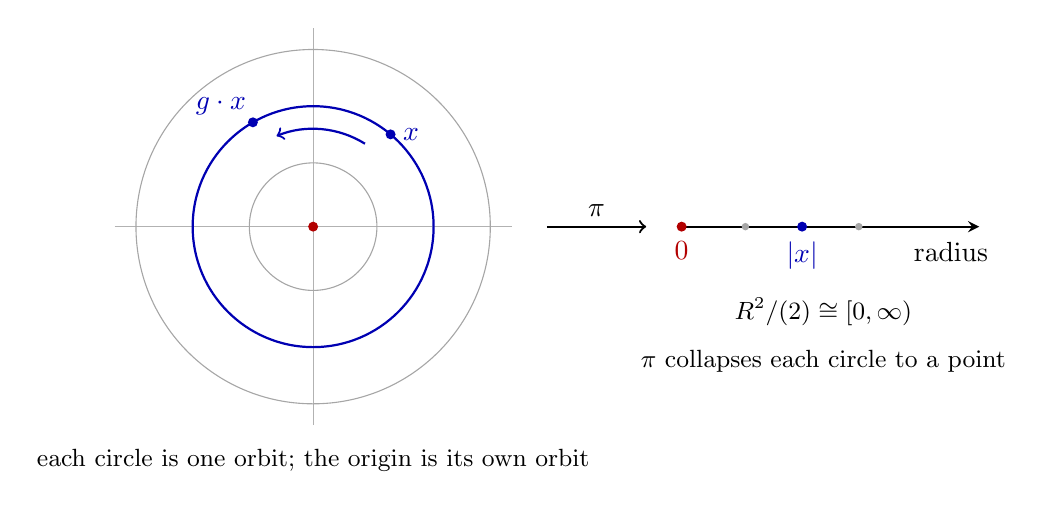
\begin{tikzpicture}[scale=0.9]
    % left panel: the plane with orbits
    \draw[gray!60] (-2.8,0) -- (2.8,0);
    \draw[gray!60] (0,-2.8) -- (0,2.8);
    \draw[gray!70] (0,0) circle (0.9);
    \draw[thick, blue!70!black] (0,0) circle (1.7);
    \draw[gray!70] (0,0) circle (2.5);
    \fill[red!70!black] (0,0) circle (2pt);
    \fill[blue!70!black] (50:1.7) circle (2pt) node[right=1pt] {$x$};
    \fill[blue!70!black] (120:1.7) circle (2pt) node[above left=-1pt] {$g \cdot x$};
    \draw[->, thick, blue!70!black] (58:1.38) arc (58:112:1.38);
    \node at (0,-3.3) {\small each circle is one orbit; the origin is its own orbit};
    % quotient arrow
    \draw[->, thick] (3.3,0) -- (4.7,0) node[midway, above] {$\pi$};
    % right panel: orbit space
    \draw[thick, -stealth] (5.2,0) -- (9.4,0);
    \fill[red!70!black] (5.2,0) circle (2pt) node[below=2pt] {$0$};
    \fill[gray!70] (6.1,0) circle (1.5pt);
    \fill[blue!70!black] (6.9,0) circle (2pt) node[below=2pt] {$|x|$};
    \fill[gray!70] (7.7,0) circle (1.5pt);
    \node[below=2pt] at (9.0,0) {radius};
    \node at (7.2,-1.2) {\small $\mathbb{R}^2/\SO(2) \cong [0,\infty)$};
    \node at (7.2,-1.9) {\small $\pi$ collapses each circle to a point};
\end{tikzpicture}
